\documentclass[12pt, a4paper]{article}

% ── Packages ────────────────────────────────────────────────────────────────
% ── Packages ────────────────────────────────────────────────────────────────
\usepackage[margin=2.5cm]{geometry}
\usepackage[T1]{fontenc}
\usepackage[utf8]{inputenc}
\usepackage{lmodern}
\usepackage{graphicx}
\usepackage{listings}
\usepackage{xcolor}
\usepackage{hyperref}
\usepackage{booktabs}
\usepackage{array}
\usepackage{tabularx}
\usepackage{fancyhdr}
\usepackage{titlesec}
\usepackage{enumitem}
\usepackage{parskip}
\usepackage{float}
\usepackage{tikz}
\usetikzlibrary{shapes.geometric, arrows.meta, positioning}


% ── Page Style ───────────────────────────────────────────────────────────────
\pagestyle{fancy}
\fancyhf{}
\rhead{EC9590 -- Network Application Design}
\lhead{Session Management Report}
\rfoot{Page \thepage}
\lfoot{University of Jaffna}

% ── Colour Definitions ───────────────────────────────────────────────────────
\definecolor{codeblue}{RGB}{0, 102, 204}
\definecolor{codegray}{RGB}{245, 245, 245}
\definecolor{codegreen}{RGB}{34, 139, 34}
\definecolor{codepurple}{RGB}{148, 0, 211}
\definecolor{codered}{RGB}{180, 0, 0}
\definecolor{uojblue}{RGB}{0, 51, 102}

% ── Code Listing Style ───────────────────────────────────────────────────────
\lstdefinestyle{javastyle}{
    backgroundcolor=\color{codegray},
    commentstyle=\color{codegreen}\itshape,
    keywordstyle=\color{codeblue}\bfseries,
    stringstyle=\color{codered},
    numberstyle=\tiny\color{gray},
    basicstyle=\ttfamily\footnotesize,
    breakatwhitespace=false,
    breaklines=true,
    captionpos=b,
    keepspaces=true,
    numbers=left,
    numbersep=8pt,
    showspaces=false,
    showstringspaces=false,
    showtabs=false,
    tabsize=2,
    frame=single,
    rulecolor=\color{gray!40},
    xleftmargin=15pt,
    language=Java
}

\lstdefinestyle{sqlstyle}{
    backgroundcolor=\color{codegray},
    commentstyle=\color{codegreen}\itshape,
    keywordstyle=\color{codepurple}\bfseries,
    stringstyle=\color{codered},
    basicstyle=\ttfamily\footnotesize,
    breaklines=true,
    frame=single,
    rulecolor=\color{gray!40},
    xleftmargin=15pt,
    language=SQL,
    morekeywords={AUTO_INCREMENT, VARCHAR, NOT, NULL, PRIMARY, KEY, UNIQUE}
}

\lstdefinestyle{httpstyle}{
    backgroundcolor=\color{codegray},
    basicstyle=\ttfamily\footnotesize,
    breaklines=true,
    breakindent=0pt,          % add this
    columns=flexible,         % add this
    frame=single,
    rulecolor=\color{gray!40},
    xleftmargin=15pt,
}

% ── Section Title Formatting ─────────────────────────────────────────────────
\titleformat{\section}
  {\Large\bfseries\color{uojblue}}{\thesection}{1em}{}[\titlerule]

\titleformat{\subsection}
  {\large\bfseries\color{uojblue!80}}{\thesubsection}{1em}{}

% ── Hyperlink Style ──────────────────────────────────────────────────────────
\hypersetup{
    colorlinks=true,
    linkcolor=uojblue,
    urlcolor=codeblue,
    pdftitle={EC9590 Lab 05-06 Session Management Report},
    pdfauthor={Dayarathna D.D.R.N.}
}

% ════════════════════════════════════════════════════════════════════════════
\begin{document}

% ── Title Page ───────────────────────────────────────────────────────────────
\begin{titlepage}
    \centering
    \vspace*{1cm}

    {\Large \textbf{Faculty of Engineering}}\\[0.3cm]
    {\large Department of Computer Engineering}\\[0.3cm]
    {\large University of Jaffna}\\[1.5cm]

    \rule{\linewidth}{0.5mm}\\[0.4cm]
    {\LARGE \textbf{EC9590: Network Application Design}}\\[0.3cm]
    {\Large Lab 05 \& 06 --- Task 02, Part 02}\\[0.3cm]
    {\huge \textbf{Session Management with Cookies}}\\[0.3cm]
    {\large Student Information Management System (SIMS)}\\
    \rule{\linewidth}{0.5mm}\\[1.5cm]

    \begin{tabular}{ll}
        \textbf{Name}       & : Dayarathna D.D.R.N. \\[0.3cm]
        \textbf{Index Number} & : 2022/E/033 \\[0.3cm]
        \textbf{Date}       & : 20 March 2026 \\[0.3cm]
        \textbf{Lecturer}   & : Dr.\ J.\ Jananie \\[0.3cm]
        \textbf{Department} & : Computer Engineering \\[0.3cm]
        \textbf{Server}     & : Apache Tomcat 10.1.52 \\[0.3cm]
        \textbf{Language}   & : Java 21 (Temurin), Jakarta EE 6 \\
        \textbf{Source Code} & : \href{https://github.com/Ravindu56/SIMS}
                             {\texttt{github.com/Ravindu56/SIMS}} \\
    \end{tabular}

    \vfill
    {\large \today}
\end{titlepage}

% ── Table of Contents ─────────────────────────────────────────────────────────
\tableofcontents
\newpage

% ════════════════════════════════════════════════════════════════════════════
\section{Introduction}

This report documents the implementation of session management with cookies
in the \textbf{Student Information Management System (SIMS)}, a web-based
application built using Jakarta Servlets, JSP, JDBC, and Apache Tomcat 10.1.

HTTP is a \textit{stateless} protocol --- each request is entirely independent
and the server retains no memory of previous interactions. Session management
bridges this gap by assigning each authenticated user a unique \textbf{Session
ID}, stored in a browser cookie and verified on every subsequent request.

The implementation covers six explicitly defined stages:

\begin{enumerate}[leftmargin=2cm]
    \item \textbf{Login} --- User submits credentials
    \item \textbf{Creation} --- Server creates a session record
    \item \textbf{Transmission} --- Server sends \texttt{Set-Cookie} header
    \item \textbf{Persistence} --- Browser attaches cookie to every request
    \item \textbf{Validation} --- Server verifies session on every page load
    \item \textbf{Termination} --- Server destroys session on logout
\end{enumerate}

% ════════════════════════════════════════════════════════════════════════════
\section{System Architecture}

The project follows the \textbf{Model-View-Controller (MVC)} architectural
pattern. The directory structure is as follows:

\begin{lstlisting}[style=httpstyle, caption={Project Structure}]
src/main/java/com/ec9590/sims/
├── model/
│   ├── Student.java          -- Student entity
│   └── User.java             -- Login user entity
├── dao/
│   ├── DBConnection.java     -- JDBC connection utility
│   ├── StudentDAO.java       -- Student CRUD operations
│   └── UserDAO.java          -- Credential validation
├── servlet/
│   ├── LoginServlet.java     -- Login (Creation + Transmission)
│   ├── LogoutServlet.java    -- Logout (Termination)
│   ├── ViewStudentServlet.java
│   ├── AddStudentServlet.java
│   ├── EditStudentServlet.java
│   ├── UpdateStudentServlet.java
│   ├── DeleteStudentServlet.java
│   └── SearchStudentServlet.java
└── filter/
    └── SessionFilter.java    -- Validation on every request
\end{lstlisting}

% ════════════════════════════════════════════════════════════════════════════
\section{Database Design}

Two tables are used in the \texttt{sims\_db} MySQL database.

\subsection{Users Table}

\begin{lstlisting}[style=sqlstyle, caption={users table DDL}]
CREATE TABLE users (
    id        INT AUTO_INCREMENT PRIMARY KEY,
    username  VARCHAR(50)  UNIQUE NOT NULL,
    password  VARCHAR(255) NOT NULL
);

-- Default admin account
INSERT INTO users (username, password) VALUES ('admin', 'admin123');
\end{lstlisting}

\subsection{Students Table}

\begin{lstlisting}[style=sqlstyle, caption={students table DDL}]
CREATE TABLE students (
    id      INT AUTO_INCREMENT PRIMARY KEY,
    reg_no  VARCHAR(20)  UNIQUE NOT NULL,
    name    VARCHAR(100) NOT NULL,
    field   VARCHAR(60)  NOT NULL,
    dob     DATE         NOT NULL,
    contact VARCHAR(15),
    email   VARCHAR(100)
);
\end{lstlisting}

% ════════════════════════════════════════════════════════════════════════════
\section{Session Management Implementation}

% ── Stage 1 ──────────────────────────────────────────────────────────────────
\subsection{Stage 1 --- Login}

\textbf{Description:} The user navigates to \texttt{/login.jsp} and submits
their username and password via an HTML form using HTTP POST.

\begin{lstlisting}[style=javastyle, caption={login.jsp -- HTML form}]
<form action="login" method="post">
    <label>Username:</label>
    <input type="text" name="username" required>

    <label>Password:</label>
    <input type="password" name="password" required>

    <button type="submit">Login</button>
</form>
\end{lstlisting}

\texttt{LoginServlet.doPost()} receives the credentials and validates them
against the database using \texttt{UserDAO.validateUser()}, which uses a
\texttt{PreparedStatement} to prevent SQL injection:

\begin{lstlisting}[style=javastyle, caption={UserDAO.java -- validateUser()}]
public User validateUser(String username, String password)
        throws SQLException {
    String sql = "SELECT * FROM users "
               + "WHERE username = ? AND password = ?";
    try (Connection con = DBConnection.getConnection();
         PreparedStatement ps = con.prepareStatement(sql)) {

        ps.setString(1, username);
        ps.setString(2, password);

        try (ResultSet rs = ps.executeQuery()) {
            if (rs.next()) {
                return new User(rs.getInt("id"),
                                rs.getString("username"),
                                rs.getString("password"));
            }
        }
    }
    return null; // invalid credentials
}
\end{lstlisting}

\begin{figure}[H]
    \centering
    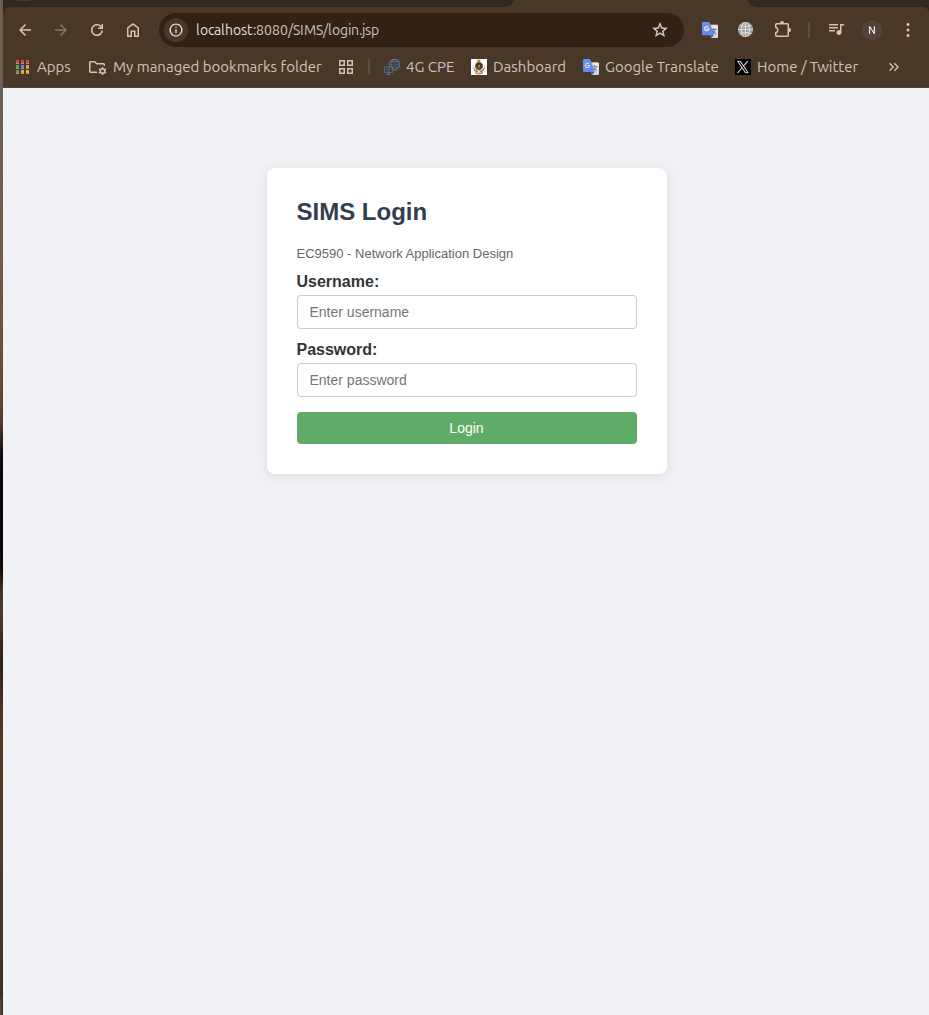
\includegraphics[width=0.85\textwidth]{screenshots/01_login_page.png}
    \caption{Login page -- user enters credentials}
    \label{fig:login}
\end{figure}


% ── Stage 2 ──────────────────────────────────────────────────────────────────
\subsection{Stage 2 --- Creation}

\textbf{Description:} Upon successful credential verification, the server
creates a new server-side session record and maps the Session ID to the
authenticated user.

\begin{lstlisting}[style=javastyle, caption={LoginServlet.java -- Session Creation}]
if (user != null) {
    // Invalidate old session to prevent session fixation attacks
    HttpSession oldSession = req.getSession(false);
    if (oldSession != null) oldSession.invalidate();

    // Create new session -- Tomcat generates a unique Session ID
    HttpSession session = req.getSession(true);

    // Map Session ID to the authenticated user
    session.setAttribute("loggedInUser", user.getUsername());

    // Set session timeout: 30 minutes of inactivity
    session.setMaxInactiveInterval(30 * 60);
\end{lstlisting}

Internally, Tomcat maintains the following mapping:

\begin{lstlisting}[style=httpstyle, caption={Tomcat internal session store}]
SessionID_ABC123  -->  { loggedInUser: "admin",
                         createdAt: 2026-03-20T10:00:00,
                         lastAccessed: 2026-03-20T10:00:00 }
\end{lstlisting}

\begin{figure}[H]
    \centering
    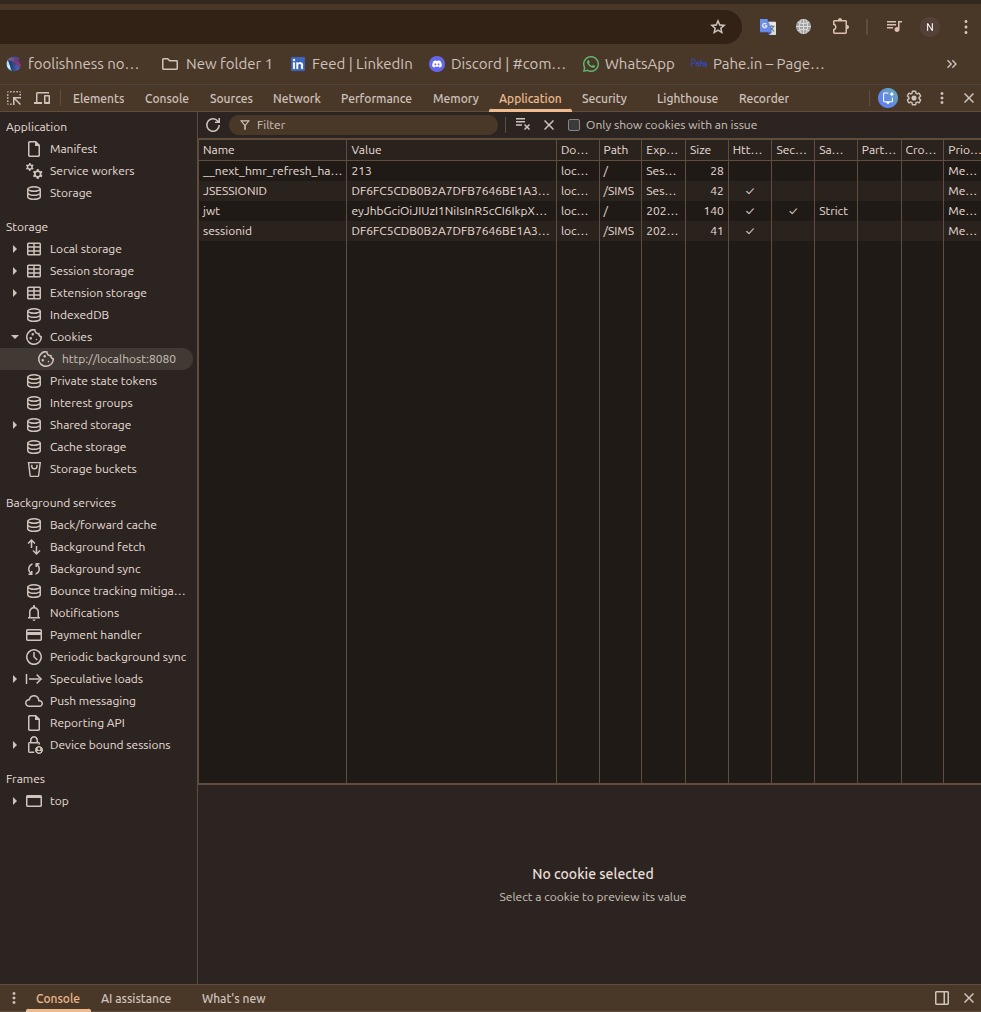
\includegraphics[width=0.85\textwidth]{screenshots/02_session_created.png}
    \caption{DevTools $\to$ Application $\to$ Cookies -- JSESSIONID created after login}
    \label{fig:creation}
\end{figure}


% ── Stage 3 ──────────────────────────────────────────────────────────────────
\subsection{Stage 3 --- Transmission}

\textbf{Description:} The server sends the Session ID to the browser via the
\texttt{Set-Cookie} HTTP response header with \texttt{HttpOnly} and
\texttt{Secure} flags.

\begin{lstlisting}[style=javastyle, caption={LoginServlet.java -- Cookie Transmission}]
// Create cookie carrying the Session ID
Cookie sessionCookie = new Cookie("sessionid", session.getId());
sessionCookie.setHttpOnly(true);   // blocks JavaScript access
sessionCookie.setSecure(false);    // set true in production (HTTPS)
sessionCookie.setPath(req.getContextPath());
sessionCookie.setMaxAge(30 * 60);  // 30 minute lifetime

// Add Set-Cookie header to HTTP response
res.addCookie(sessionCookie);
res.sendRedirect(req.getContextPath() + "/viewStudents");
\end{lstlisting}

The resulting HTTP response header is:

\begin{lstlisting}[style=httpstyle, caption={HTTP Response Header}]
HTTP/1.1 302 Found
Set-Cookie: sessionid=ABC123XYZ; HttpOnly; Path=/SIMS; Max-Age=1800
Set-Cookie: JSESSIONID=ABC123XYZ; HttpOnly; Path=/SIMS
Location: http://localhost:8080/SIMS/viewStudents
\end{lstlisting}

\noindent\textbf{Note on \texttt{Secure} flag:} The \texttt{Secure} flag is
set to \texttt{false} during development because the server runs on plain
HTTP. In a production environment with HTTPS/TLS, this must be \texttt{true}
to prevent the cookie from being transmitted over unencrypted connections.

\begin{figure}[H]
    \centering
    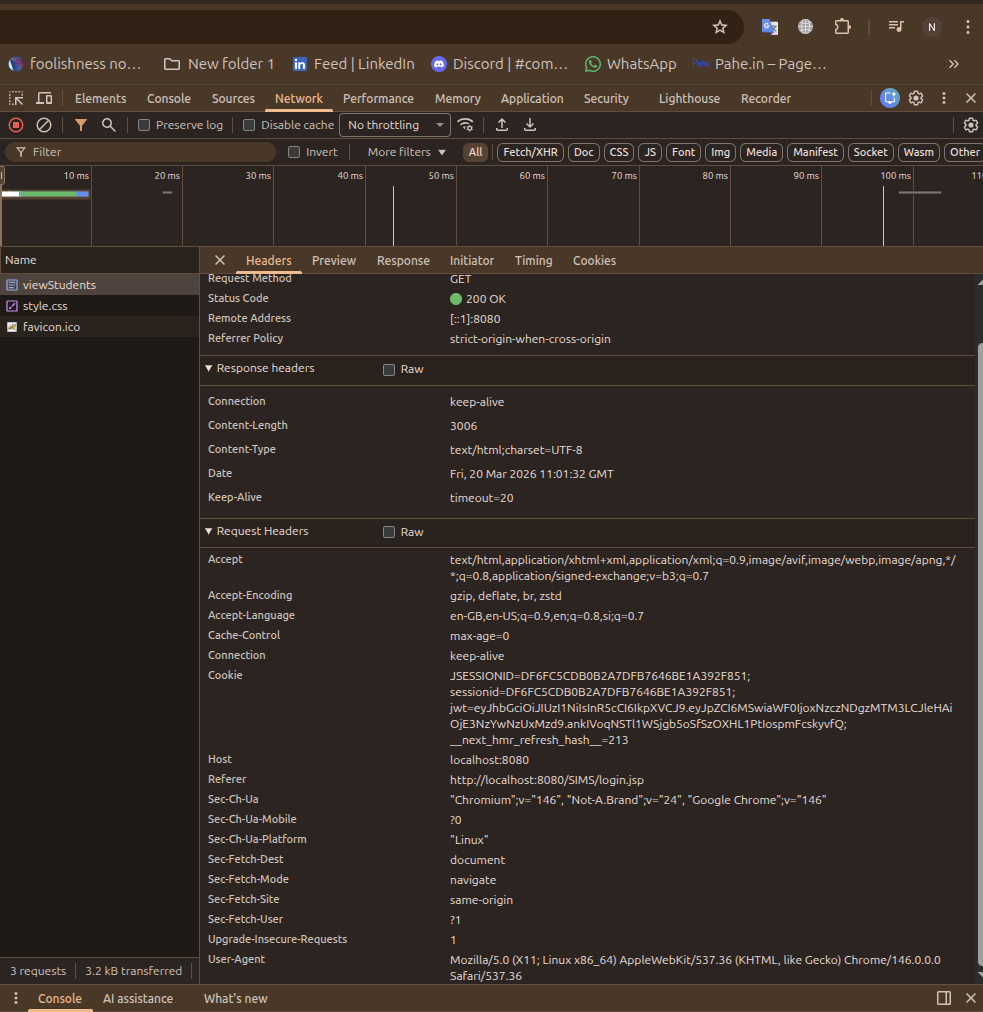
\includegraphics[width=0.85\textwidth]{screenshots/03_set_cookie_header.png}
    \caption{DevTools $\to$ Network $\to$ login POST $\to$ Response Headers -- Set-Cookie}
    \label{fig:transmission}
\end{figure}

% ── Stage 4 ──────────────────────────────────────────────────────────────────
\subsection{Stage 4 --- Persistence}

\textbf{Description:} The browser stores the cookie and automatically attaches
it to every subsequent HTTP request to the server.

After login, every request includes the cookie in its headers:

\begin{lstlisting}[style=httpstyle, caption={HTTP Request Header -- Cookie sent automatically}]
GET /SIMS/viewStudents HTTP/1.1
Host: localhost:8080
Cookie: sessionid=ABC123XYZ; JSESSIONID=ABC123XYZ
\end{lstlisting}

The session attribute is available on every protected JSP page:

\begin{lstlisting}[style=javastyle, caption={viewStudents.jsp -- Session persistence demonstrated}]
<!-- Session attribute accessible on every protected page -->
Welcome, <strong><%= session.getAttribute("loggedInUser") %></strong>
<a href="<%= request.getContextPath() %>/logout">Logout</a>
\end{lstlisting}

\begin{figure}[H]
    \centering
    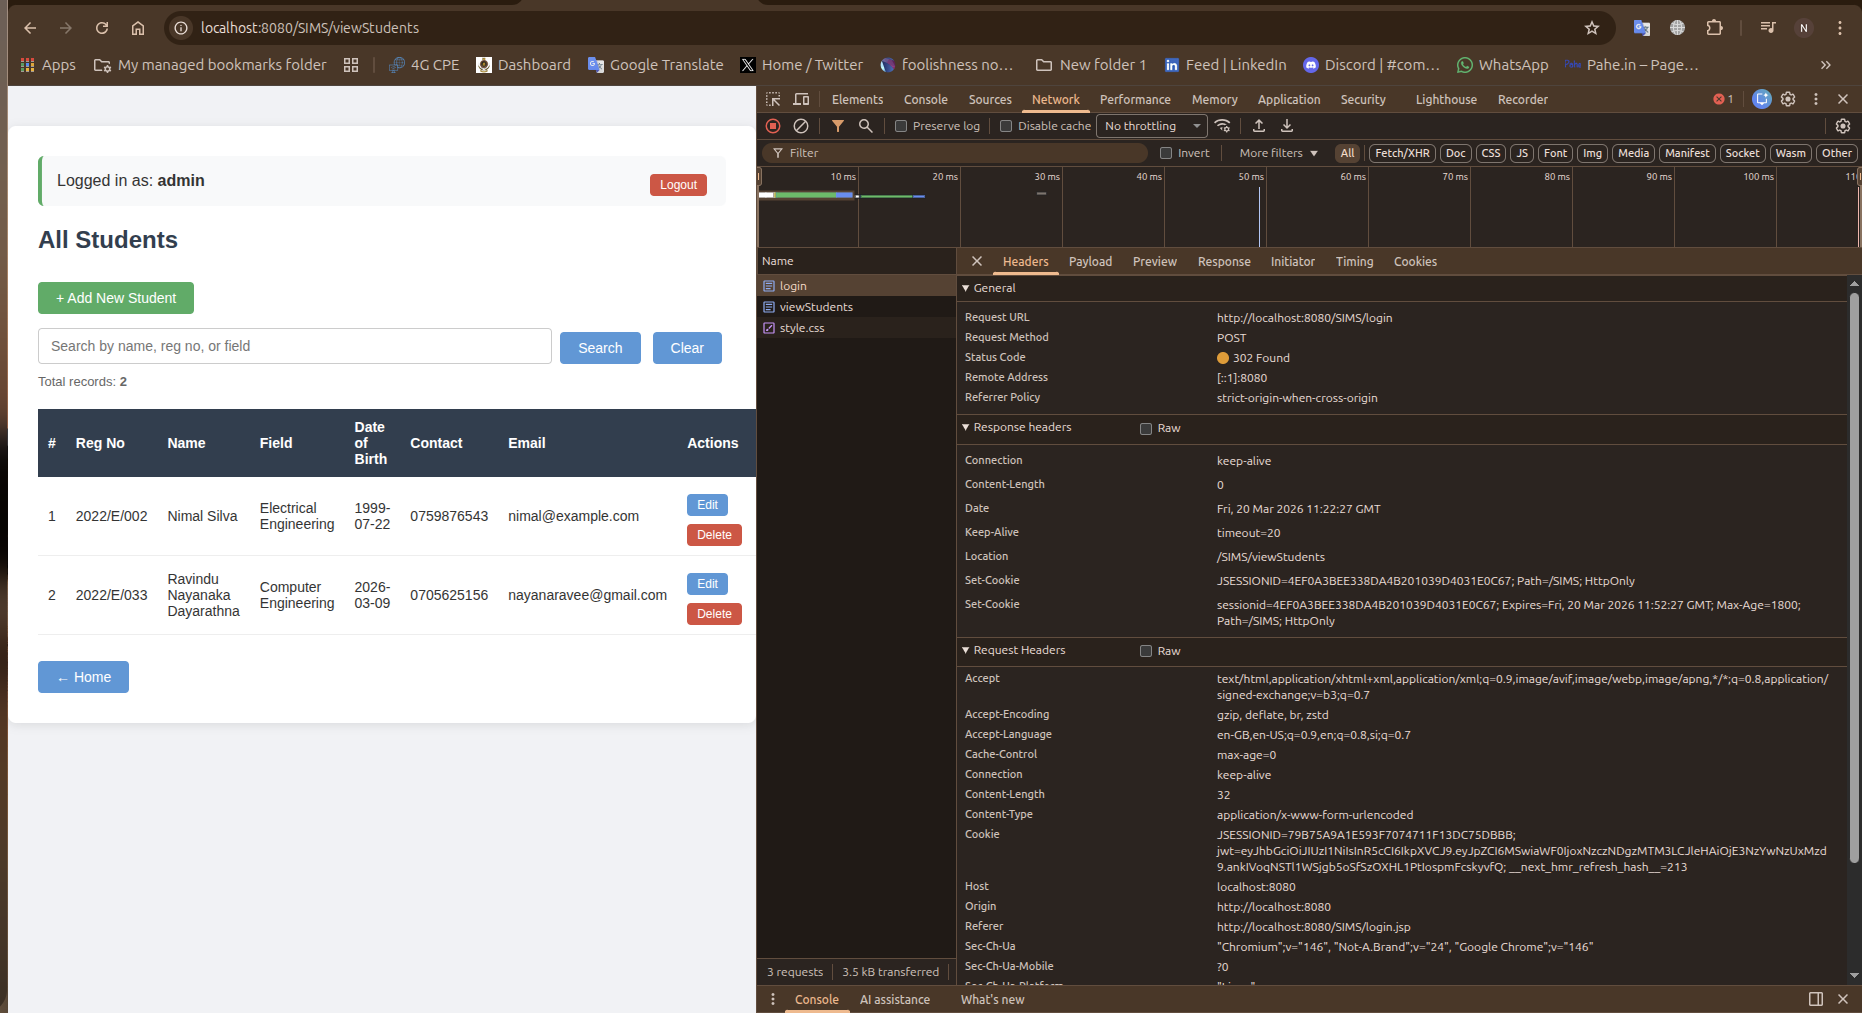
\includegraphics[width=0.85\textwidth]{screenshots/04_persistence.png}
    \caption{View Students page showing ``Welcome, admin'' -- cookie sent in Request Headers}
    \label{fig:persistence}
\end{figure}


% ── Stage 5 ──────────────────────────────────────────────────────────────────
\subsection{Stage 5 --- Validation}

\textbf{Description:} For every request to a protected resource, the server
checks whether a valid session exists before allowing access.

This is implemented as a Jakarta Servlet \texttt{Filter}, which intercepts
every request \textit{before} it reaches any Servlet:

\begin{lstlisting}[style=javastyle, caption={SessionFilter.java -- Validation on every request}]
@WebFilter(urlPatterns = {
    "/viewStudents", "/addStudent", "/editStudent",
    "/updateStudent", "/deleteStudent", "/searchStudents",
    "/addStudent.jsp", "/updateStudent.jsp",
    "/viewStudents.jsp", "/index.jsp"
})
public class SessionFilter implements Filter {

    @Override
    public void doFilter(ServletRequest request,
                         ServletResponse response,
                         FilterChain chain)
            throws IOException, ServletException {

        HttpServletRequest  req = (HttpServletRequest)  request;
        HttpServletResponse res = (HttpServletResponse) response;

        // Retrieve existing session -- do NOT create a new one
        HttpSession session = req.getSession(false);

        boolean isLoggedIn = (session != null)
                          && (session.getAttribute("loggedInUser")
                              != null);

        if (isLoggedIn) {
            // Valid session -- allow request to proceed
            chain.doFilter(request, response);
        } else {
            // No valid session -- block and redirect to login
            res.sendRedirect(
                req.getContextPath() + "/login.jsp");
        }
    }
}
\end{lstlisting}

\begin{figure}[H]
    \centering
    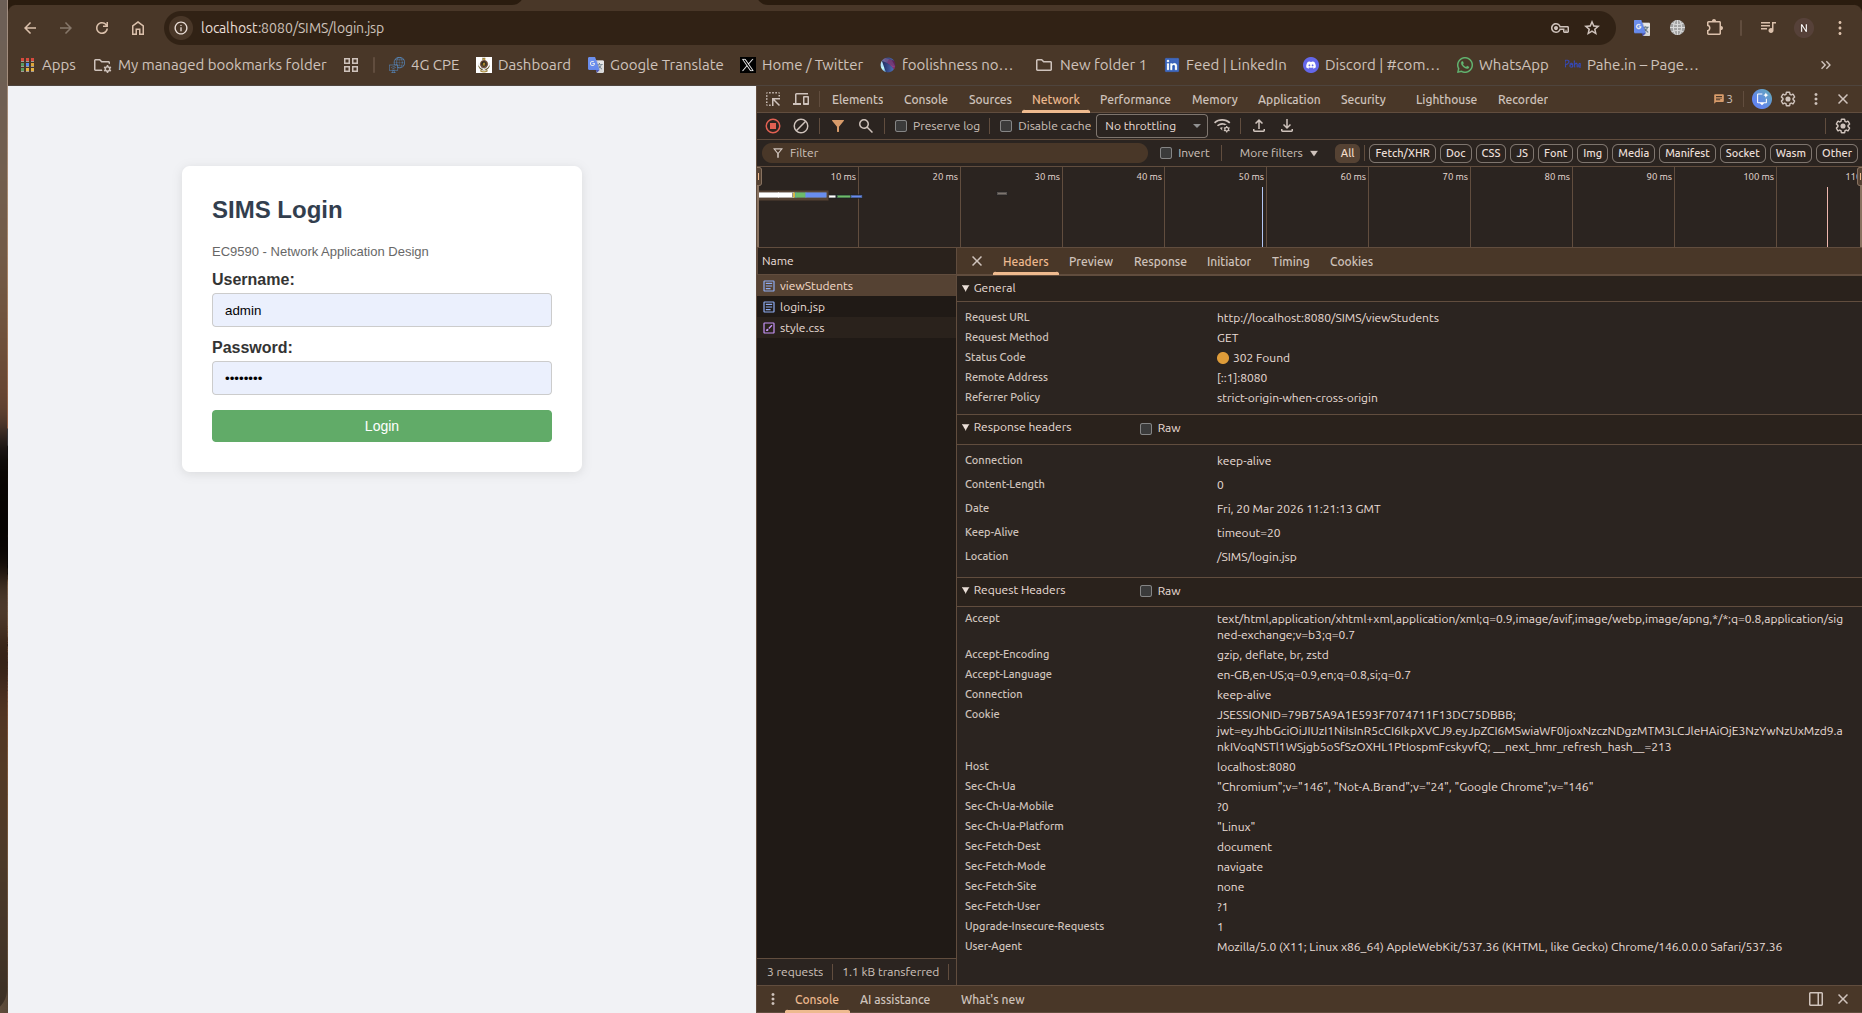
\includegraphics[width=0.85\textwidth]{screenshots/05_validation_redirect.png}
    \caption{Accessing \texttt{/viewStudents} without login redirects to login page}
    \label{fig:validation}
\end{figure}


% ── Stage 6 ──────────────────────────────────────────────────────────────────
\subsection{Stage 6 --- Termination}

\textbf{Description:} When the user clicks Logout, the server destroys the
session data and instructs the browser to delete the cookie.

\begin{lstlisting}[style=javastyle, caption={LogoutServlet.java -- Session Termination}]
@WebServlet("/logout")
public class LogoutServlet extends HttpServlet {

    @Override
    protected void doGet(HttpServletRequest req,
                         HttpServletResponse res)
            throws ServletException, IOException {

        // Step 1: Destroy the server-side session record
        HttpSession session = req.getSession(false);
        if (session != null) {
            session.invalidate(); // removes SessionID -> user mapping
        }

        // Step 2: Delete sessionid cookie from browser
        Cookie killCookie = new Cookie("sessionid", "");
        killCookie.setMaxAge(0); // MaxAge=0 deletes the cookie
        killCookie.setPath(req.getContextPath());
        res.addCookie(killCookie);

        // Step 3: Delete JSESSIONID cookie from browser
        Cookie killJSession = new Cookie("JSESSIONID", "");
        killJSession.setMaxAge(0);
        killJSession.setPath(req.getContextPath());
        res.addCookie(killJSession);

        // Step 4: Redirect to login page
        res.sendRedirect(req.getContextPath() + "/login.jsp");
    }
}
\end{lstlisting}

The HTTP response after logout:

\begin{lstlisting}[style=httpstyle, caption={HTTP Response Header -- Cookie deletion}]
HTTP/1.1 302 Found
Set-Cookie: sessionid=; Max-Age=0; Path=/SIMS
Set-Cookie: JSESSIONID=; Max-Age=0; Path=/SIMS
Location: http://localhost:8080/SIMS/login.jsp
\end{lstlisting}

\begin{figure}[H]
    \centering
    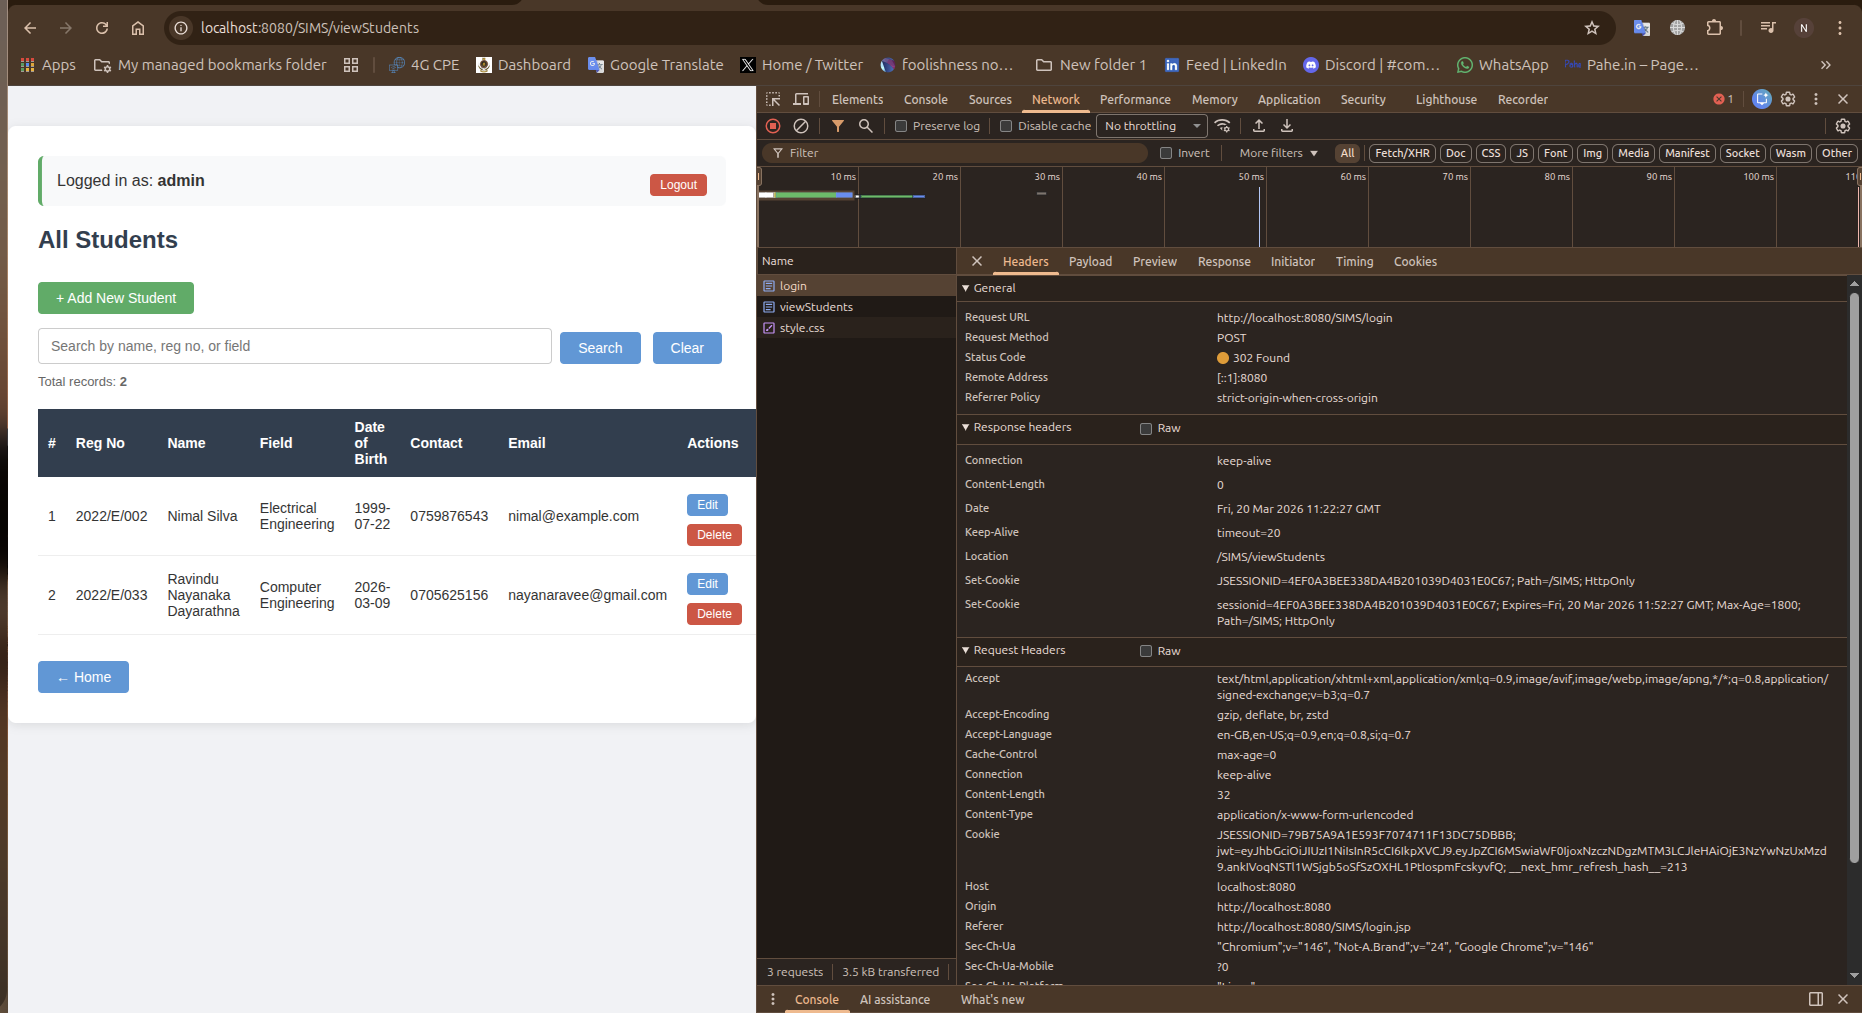
\includegraphics[width=0.85\textwidth]{screenshots/06_termination.png}
    \caption{DevTools $\to$ Network $\to$ logout -- Set-Cookie with Max-Age=0}
    \label{fig:termination}
\end{figure}


% ════════════════════════════════════════════════════════════════════════════
\section{Session Lifecycle Diagram}

\begin{figure}[H]
\centering
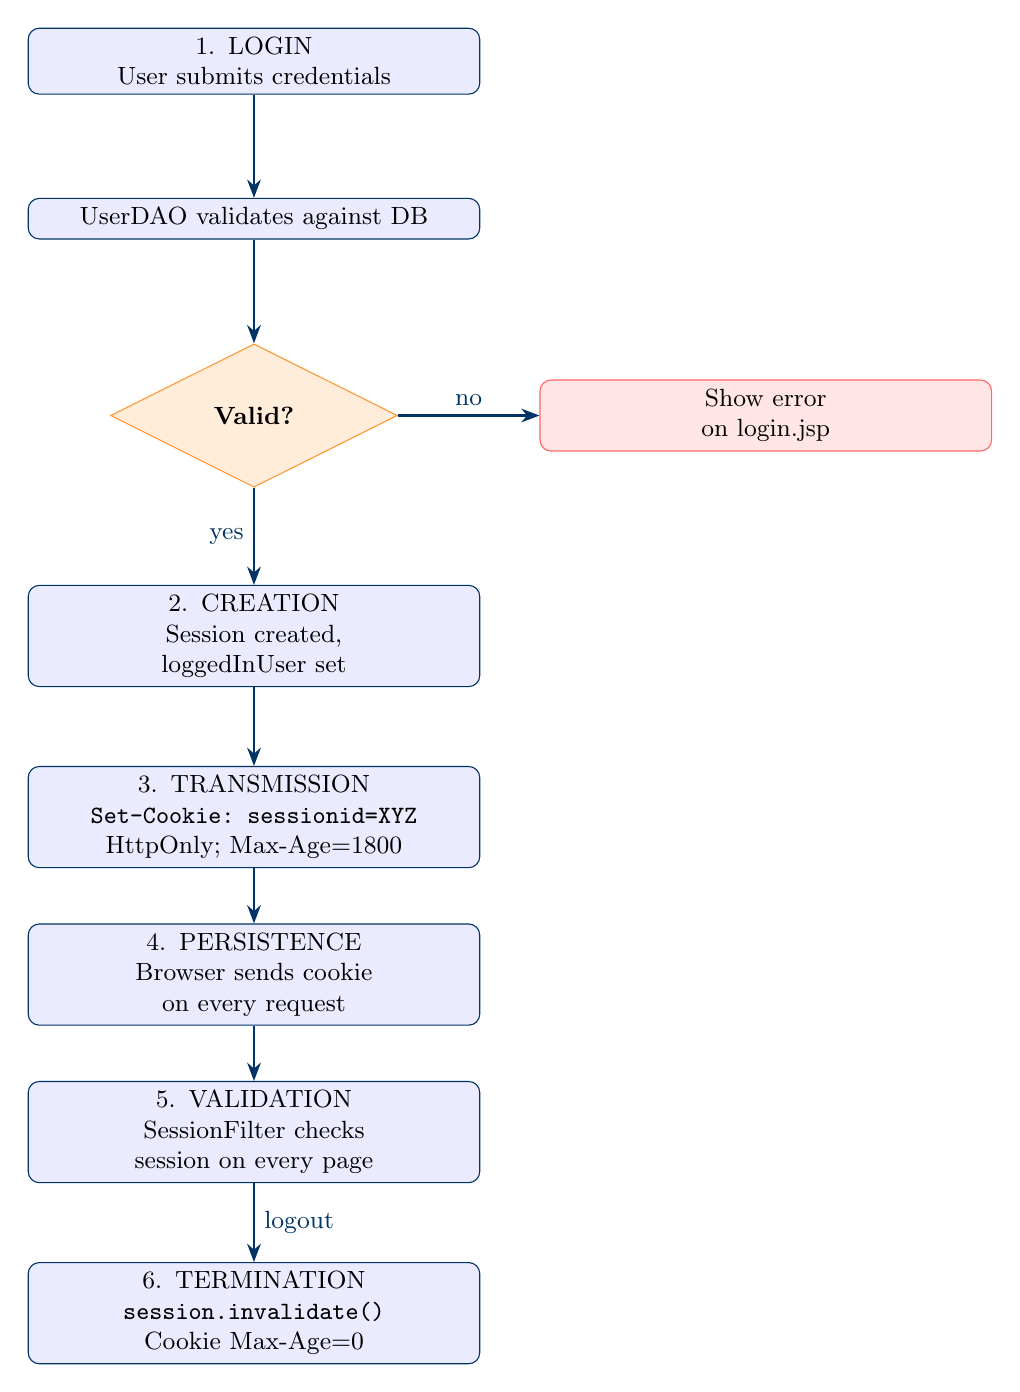
\begin{tikzpicture}[
    node distance=2.0cm,              % increased from 1.4cm
    box/.style={rectangle, rounded corners, draw=uojblue,
                fill=blue!8, text width=5.5cm,
                align=center, minimum height=0.2cm,
                font=\small},
    decision/.style={diamond, draw=orange!80, fill=orange!15,
                     text width=2.5cm, align=center,
                     aspect=2,        % makes diamond wider
                     font=\small\bfseries},
    arrow/.style={-{Stealth}, thick, color=uojblue}
]

\node (login)    [box]                                {1. LOGIN\\User submits credentials};
\node (validate) [box, below of=login]                {UserDAO validates against DB};
\node (dec)      [decision, below of=validate,
                  yshift=-0.5cm]                      {Valid?};
\node (create)   [box, below of=dec, yshift=-0.8cm]   {2. CREATION\\Session created,\\loggedInUser set};
\node (transmit) [box, below of=create, yshift=-0.3cm]{3. TRANSMISSION\\\texttt{Set-Cookie: sessionid=XYZ}\\HttpOnly; Max-Age=1800};
\node (persist)  [box, below of=transmit]             {4. PERSISTENCE\\Browser sends cookie\\on every request};
\node (filter)   [box, below of=persist]              {5. VALIDATION\\SessionFilter checks\\session on every page};
\node (logout)   [box, below of=filter, yshift=-0.3cm]               {6. TERMINATION\\\texttt{session.invalidate()}\\Cookie Max-Age=0};

\node (error)    [box, right of=dec, xshift=4.5cm,
                  fill=red!10, draw=red!60]            {Show error\\on login.jsp};

\draw [arrow] (login)    -- (validate);
\draw [arrow] (validate) -- (dec);
\draw [arrow] (dec)      -- node[left]{\small yes}  (create);
\draw [arrow] (dec)      -- node[above]{\small no}  (error);
\draw [arrow] (create)   -- (transmit);
\draw [arrow] (transmit) -- (persist);
\draw [arrow] (persist)  -- (filter);
\draw [arrow] (filter)   -- node[right]{\small logout} (logout);
\end{tikzpicture}
\caption{Complete Session Management Lifecycle in SIMS}
\end{figure}

% ════════════════════════════════════════════════════════════════════════════
\section{Security Considerations}

\begin{table}[H]
\centering
\renewcommand{\arraystretch}{1.4}
\begin{tabularx}{\textwidth}{>{\bfseries}lX}
\toprule
Security Concern & Implementation \\
\midrule
SQL Injection       & \texttt{PreparedStatement} used in all database queries \\
Session Fixation    & Old session invalidated before creating a new one on login \\
XSS Cookie Theft    & \texttt{HttpOnly} flag prevents JavaScript from reading the cookie \\
HTTPS Enforcement   & \texttt{Secure} flag to be enabled in production with TLS \\
Session Timeout     & 30-minute inactivity timeout configured via
                      \texttt{setMaxInactiveInterval()} \\
Unauthorised Access & \texttt{SessionFilter} blocks all unauthenticated requests
                      to protected URLs \\
\bottomrule
\end{tabularx}
\caption{Security Measures Implemented}
\end{table}

% ════════════════════════════════════════════════════════════════════════════
\section{Summary Table}

\begin{table}[H]
\centering
\renewcommand{\arraystretch}{1.4}
\begin{tabularx}{\textwidth}{llX}
\toprule
\textbf{Stage} & \textbf{Key File} & \textbf{Key Code} \\
\midrule
Login        & \texttt{LoginServlet.java}   & \texttt{req.getParameter("username")} \\
Creation     & \texttt{LoginServlet.java}   & \texttt{req.getSession(true)} +
                                             \texttt{setAttribute()} \\
Transmission & \texttt{LoginServlet.java}   & \texttt{new Cookie("sessionid", session.getId())} \\
Persistence  & \texttt{viewStudents.jsp}    & \texttt{session.getAttribute("loggedInUser")} \\
Validation   & \texttt{SessionFilter.java}  & \texttt{req.getSession(false)} + null check \\
Termination  & \texttt{LogoutServlet.java}  & \texttt{session.invalidate()} +
                                             \texttt{cookie.setMaxAge(0)} \\
\bottomrule
\end{tabularx}
\caption{Session Management Stage Summary}
\end{table}

% ════════════════════════════════════════════════════════════════════════════
\section{Conclusion}

The SIMS application successfully implements all six stages of cookie-based
session management as specified in the lab requirements. The
\texttt{SessionFilter} provides centralised validation on every protected
request, the \texttt{LoginServlet} handles secure session creation and cookie
transmission, and the \texttt{LogoutServlet} ensures complete session
termination on both the server and client sides.

The implementation demonstrates a foundational understanding of how stateful
web sessions are managed over the inherently stateless HTTP protocol, and
reflects the same mechanisms used internally by production-grade frameworks
such as Spring Security.

\end{document}
